% Generato da `kbench thesis` — non modificare a mano.
% Rigenerare con: kbench thesis --run-dir runs/big

\begin{figure}[htbp]
  \centering
  \begin{subfigure}[b]{\textwidth}
    \centering
    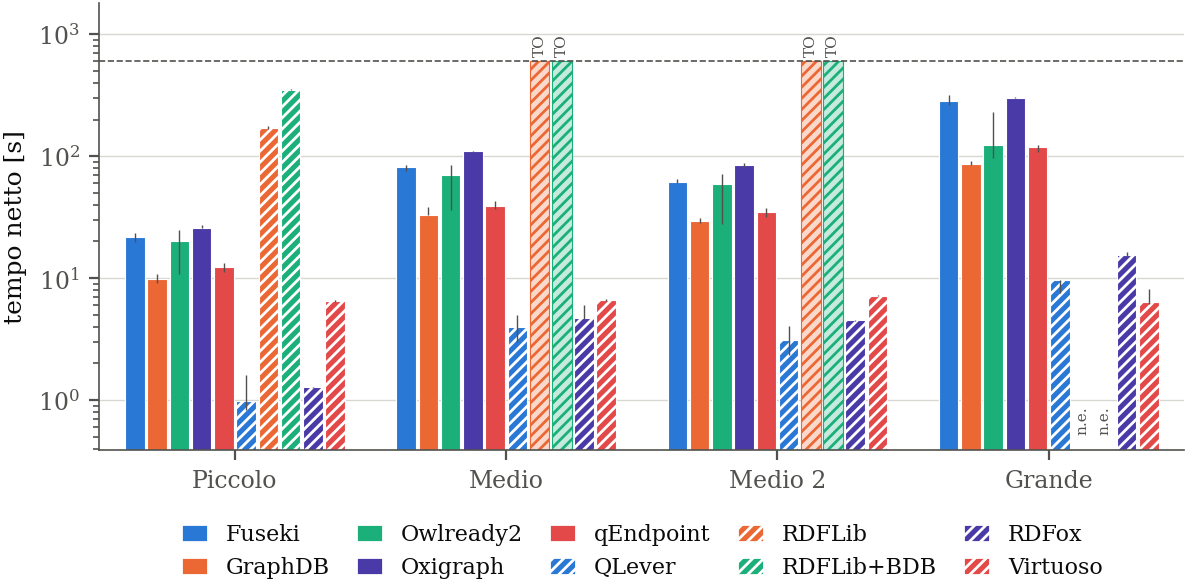
\includegraphics[width=\textwidth]{images/plots/q_select_all.png}
    \caption{Query \emph{Seleziona tutto}.}
    \label{fig:q_select_all}
  \end{subfigure}
  \\[1.5ex]
  \begin{subfigure}[b]{\textwidth}
    \centering
    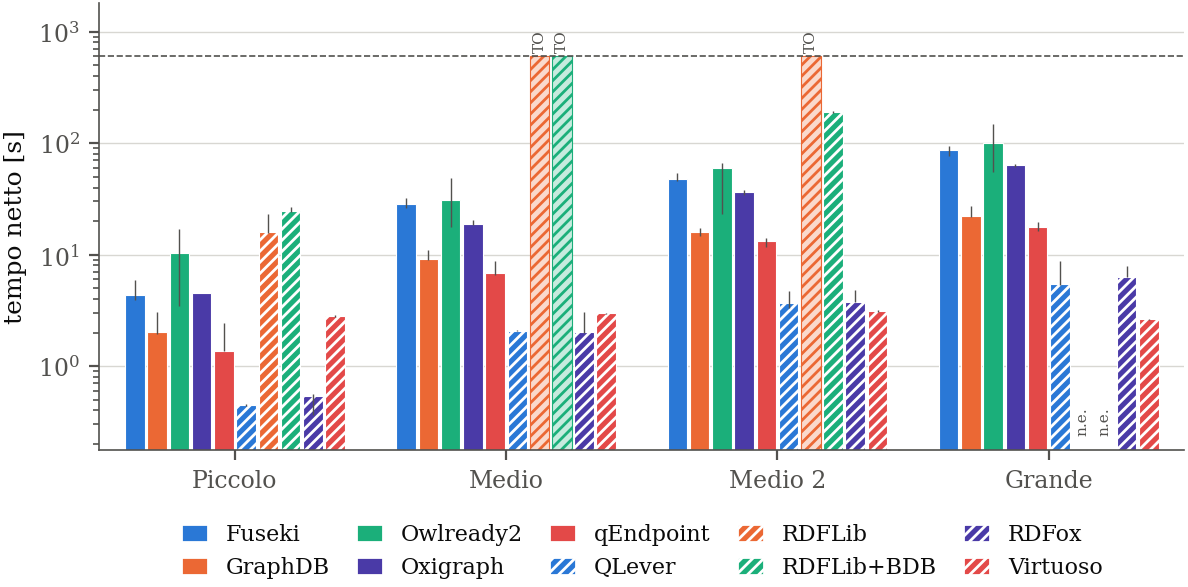
\includegraphics[width=\textwidth]{images/plots/q_scalar_max_x.png}
    \caption{Query \emph{Scalare}.}
    \label{fig:q_scalar_max_x}
  \end{subfigure}
  \caption{Confronto fra i motori per singola query, raggruppati per dataset (1 di 4). I tempi sono mediane al netto della latenza base del motore, in scala logaritmica; le barre verticali indicano l'intervallo fra minimo e massimo; le barre appoggiate al limite inferiore dell'asse corrispondono a tempi non distinguibili dalla latenza base (sotto il millisecondo). \textsf{TO} indica il superamento del timeout, \textsf{n.d.} una query non applicabile al dataset, \textsf{n.e.} una misurazione non eseguita.}
  \label{fig:queries_1}
\end{figure}

\begin{figure}[htbp]
  \centering
  \begin{subfigure}[b]{\textwidth}
    \centering
    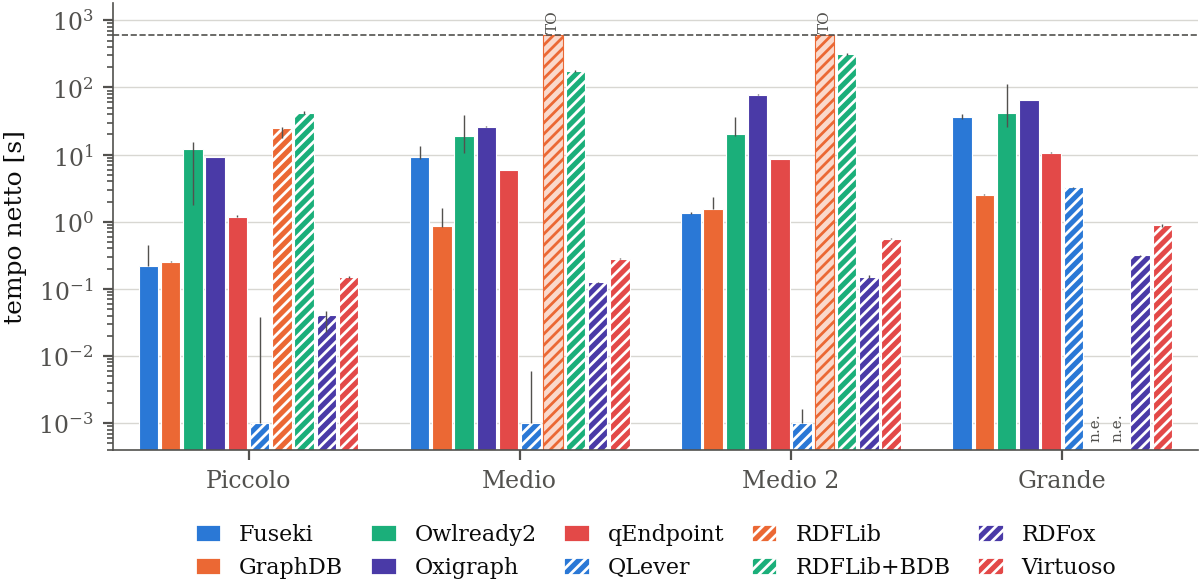
\includegraphics[width=\textwidth]{images/plots/q_select_points_in_object.png}
    \caption{Query \emph{Punti nell'oggetto}.}
    \label{fig:q_select_points_in_object}
  \end{subfigure}
  \\[1.5ex]
  \begin{subfigure}[b]{\textwidth}
    \centering
    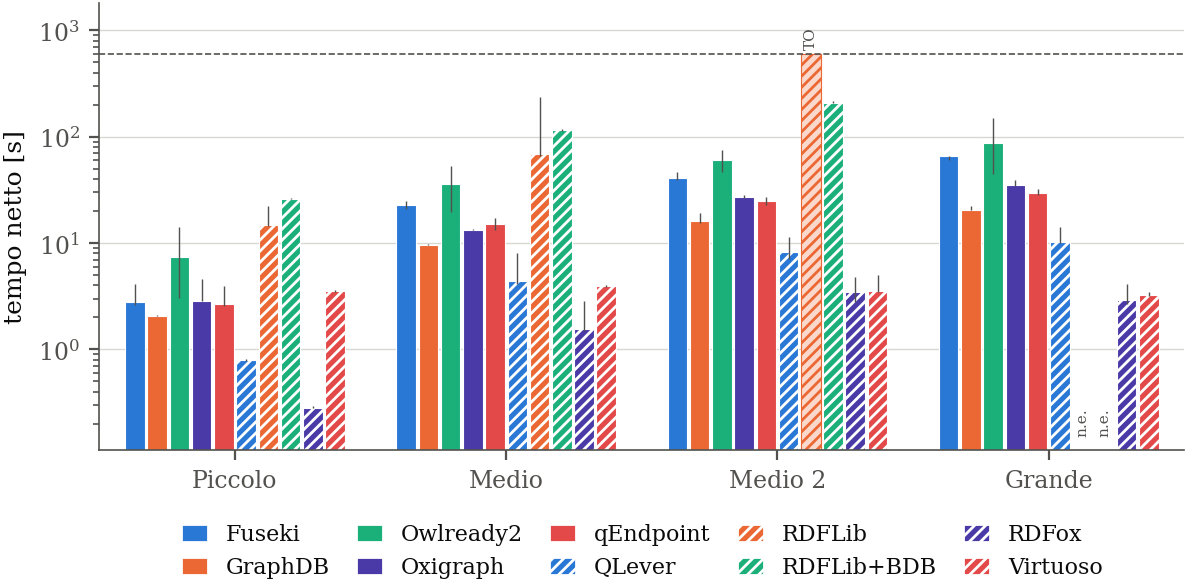
\includegraphics[width=\textwidth]{images/plots/q_instance_segmentation.png}
    \caption{Query \emph{Segmentazione delle istanze}.}
    \label{fig:q_instance_segmentation}
  \end{subfigure}
  \caption{Confronto fra i motori per singola query, raggruppati per dataset (2 di 4). Notazione come nella figura~\ref{fig:queries_1}.}
  \label{fig:queries_2}
\end{figure}

\begin{figure}[htbp]
  \centering
  \begin{subfigure}[b]{\textwidth}
    \centering
    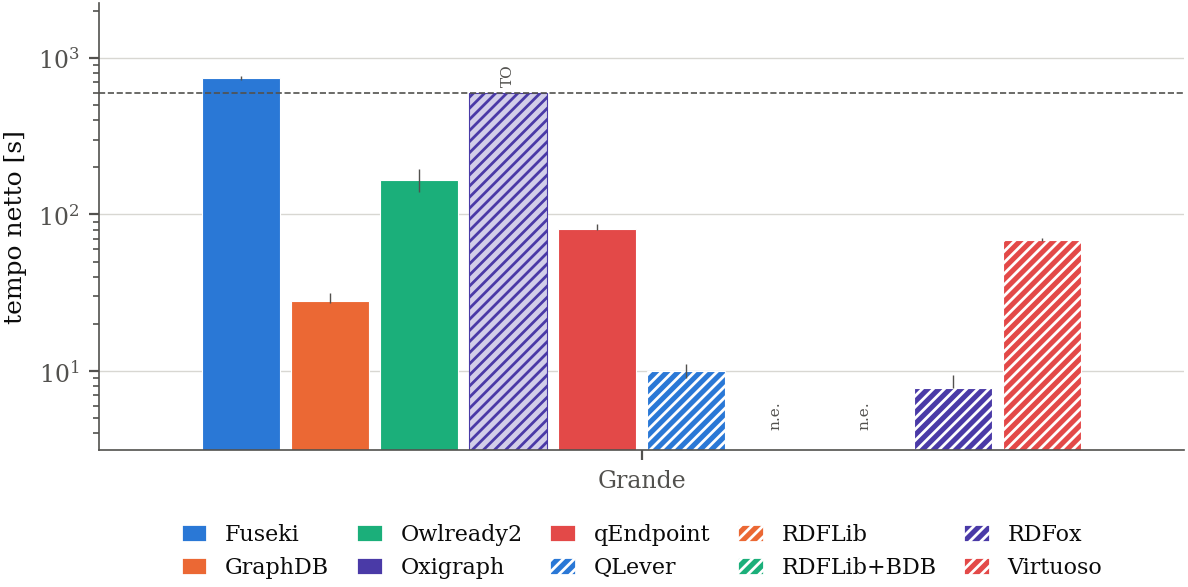
\includegraphics[width=\textwidth]{images/plots/q_chained_segmentation.png}
    \caption{Query \emph{Segmentazione tassonomica}.}
    \label{fig:q_chained_segmentation}
  \end{subfigure}
  \\[1.5ex]
  \begin{subfigure}[b]{\textwidth}
    \centering
    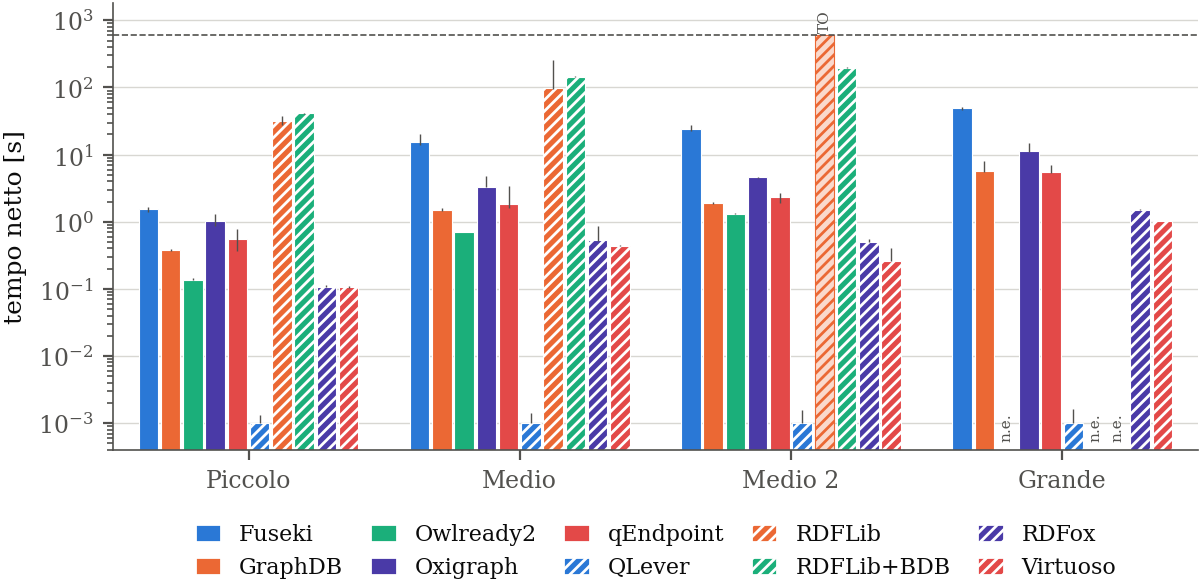
\includegraphics[width=\textwidth]{images/plots/q_max_lod.png}
    \caption{Query \emph{LOD massimo}.}
    \label{fig:q_max_lod}
  \end{subfigure}
  \caption{Confronto fra i motori per singola query, raggruppati per dataset (3 di 4). Notazione come nella figura~\ref{fig:queries_1}.}
  \label{fig:queries_3}
\end{figure}

\begin{figure}[htbp]
  \centering
  \begin{subfigure}[b]{\textwidth}
    \centering
    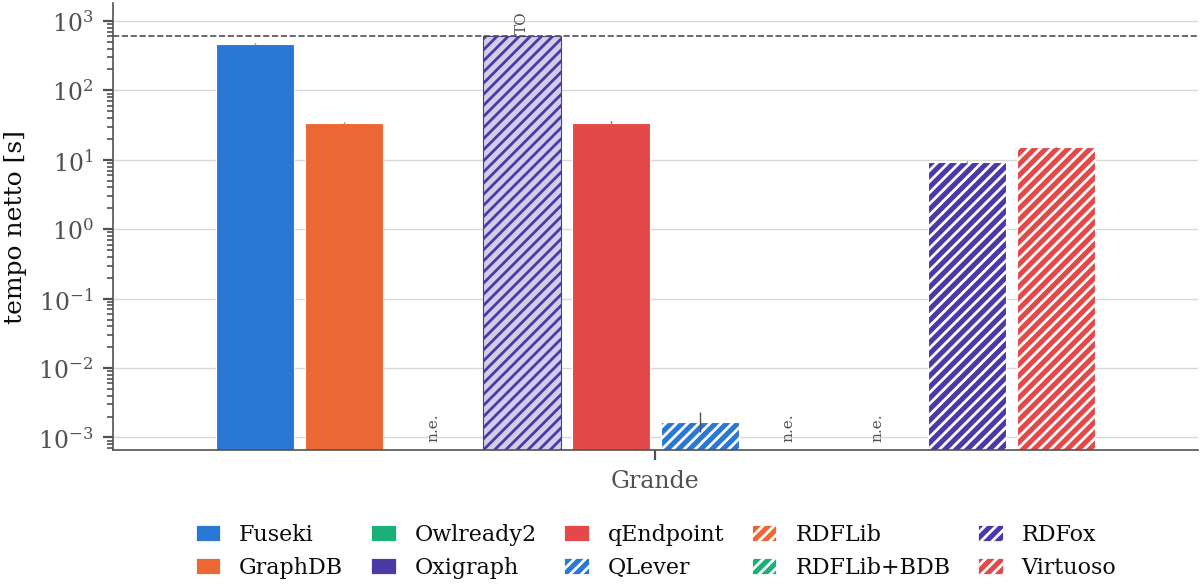
\includegraphics[width=\textwidth]{images/plots/q_taxonomical_hierarchy.png}
    \caption{Query \emph{Gerarchia tassonomica}.}
    \label{fig:q_taxonomical_hierarchy}
  \end{subfigure}
  \\[1.5ex]
  \begin{subfigure}[b]{\textwidth}
    \centering
    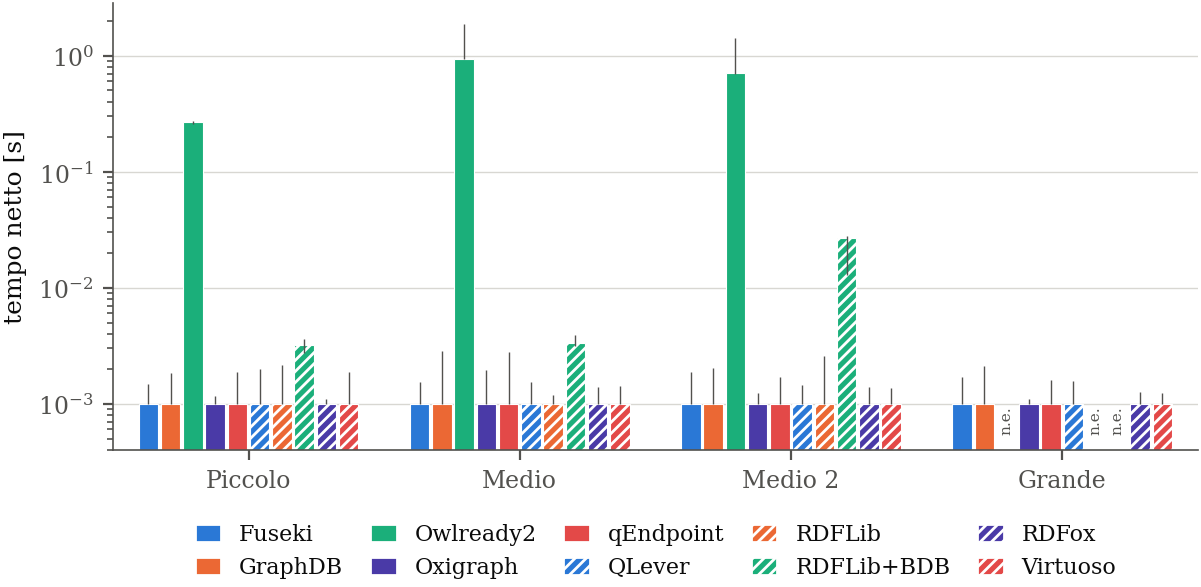
\includegraphics[width=\textwidth]{images/plots/q_avg_height.png}
    \caption{Query \emph{Altezza media}.}
    \label{fig:q_avg_height}
  \end{subfigure}
  \caption{Confronto fra i motori per singola query, raggruppati per dataset (4 di 4). Notazione come nella figura~\ref{fig:queries_1}.}
  \label{fig:queries_4}
\end{figure}

\begin{figure}[htbp]
  \centering
  \begin{subfigure}[b]{\textwidth}
    \centering
    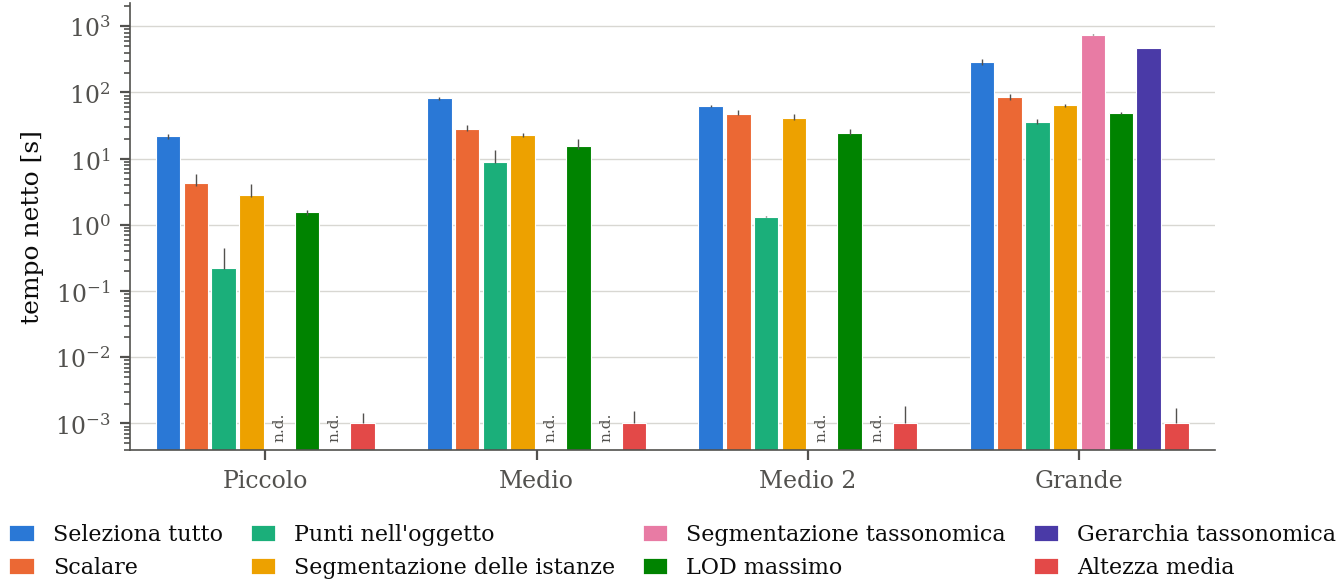
\includegraphics[width=\textwidth]{images/plots/e_fuseki.png}
    \caption{Fuseki.}
    \label{fig:e_fuseki}
  \end{subfigure}
  \\[1.5ex]
  \begin{subfigure}[b]{\textwidth}
    \centering
    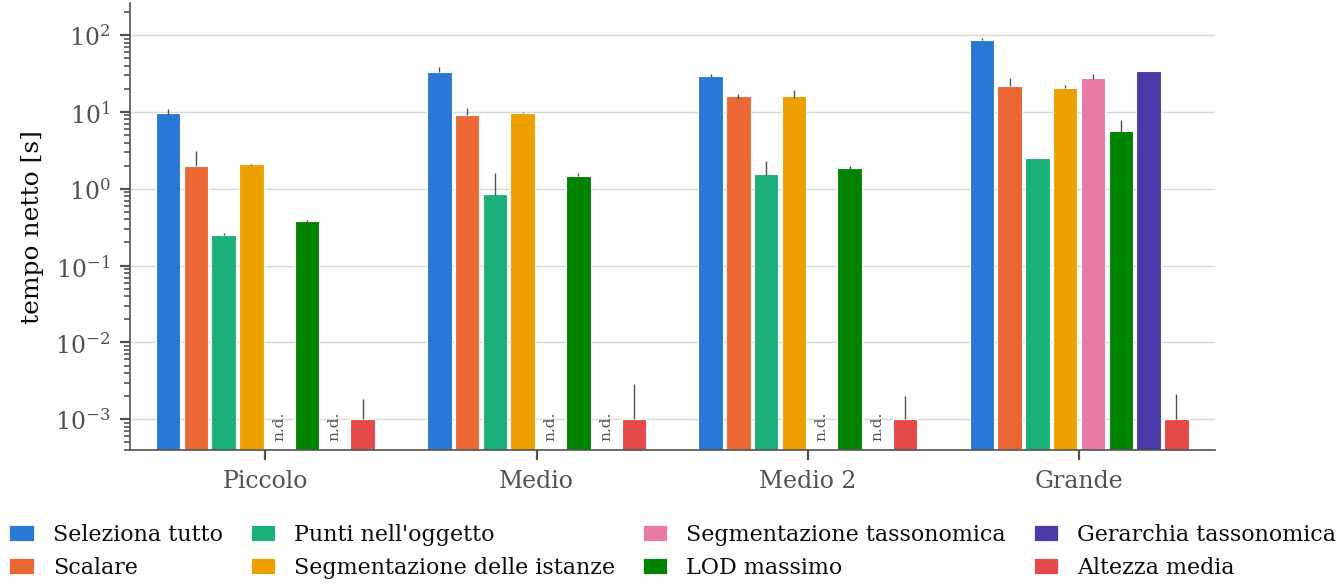
\includegraphics[width=\textwidth]{images/plots/e_graphdb.png}
    \caption{GraphDB.}
    \label{fig:e_graphdb}
  \end{subfigure}
  \caption{Confronto fra le query per singolo motore, raggruppate per dataset (1 di 5). I tempi sono mediane al netto della latenza base del motore, in scala logaritmica; le barre verticali indicano l'intervallo fra minimo e massimo; le barre appoggiate al limite inferiore dell'asse corrispondono a tempi non distinguibili dalla latenza base (sotto il millisecondo). \textsf{TO} indica il superamento del timeout, \textsf{n.d.} una query non applicabile al dataset, \textsf{n.e.} una misurazione non eseguita.}
  \label{fig:engines_1}
\end{figure}

\begin{figure}[htbp]
  \centering
  \begin{subfigure}[b]{\textwidth}
    \centering
    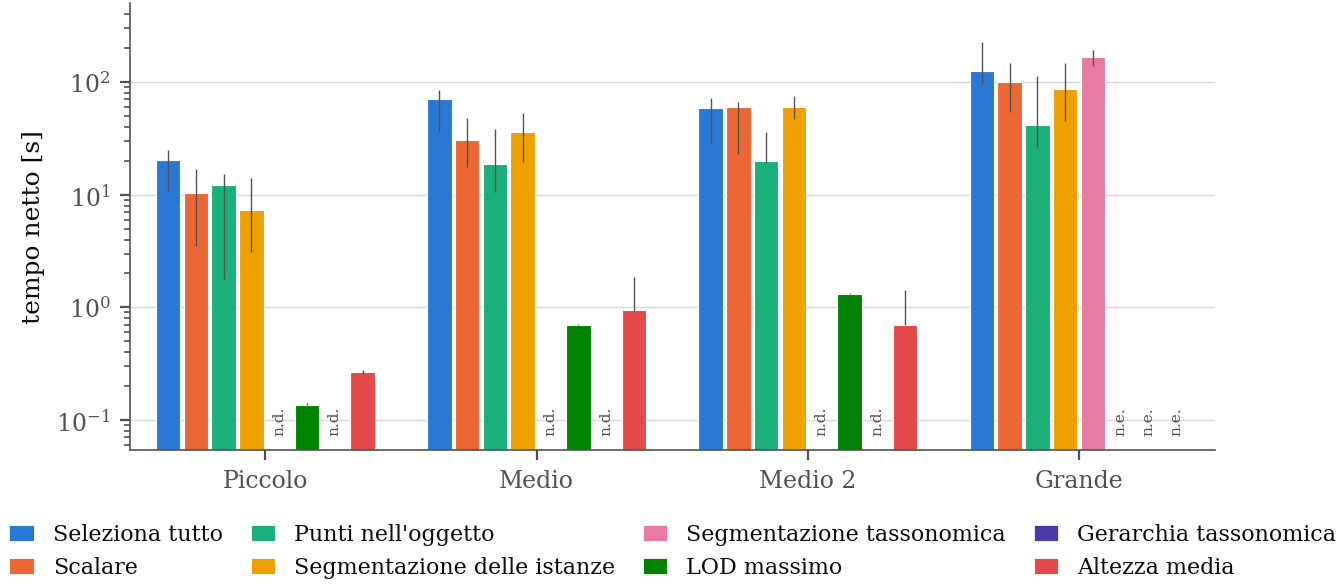
\includegraphics[width=\textwidth]{images/plots/e_owlready2.png}
    \caption{Owlready2.}
    \label{fig:e_owlready2}
  \end{subfigure}
  \\[1.5ex]
  \begin{subfigure}[b]{\textwidth}
    \centering
    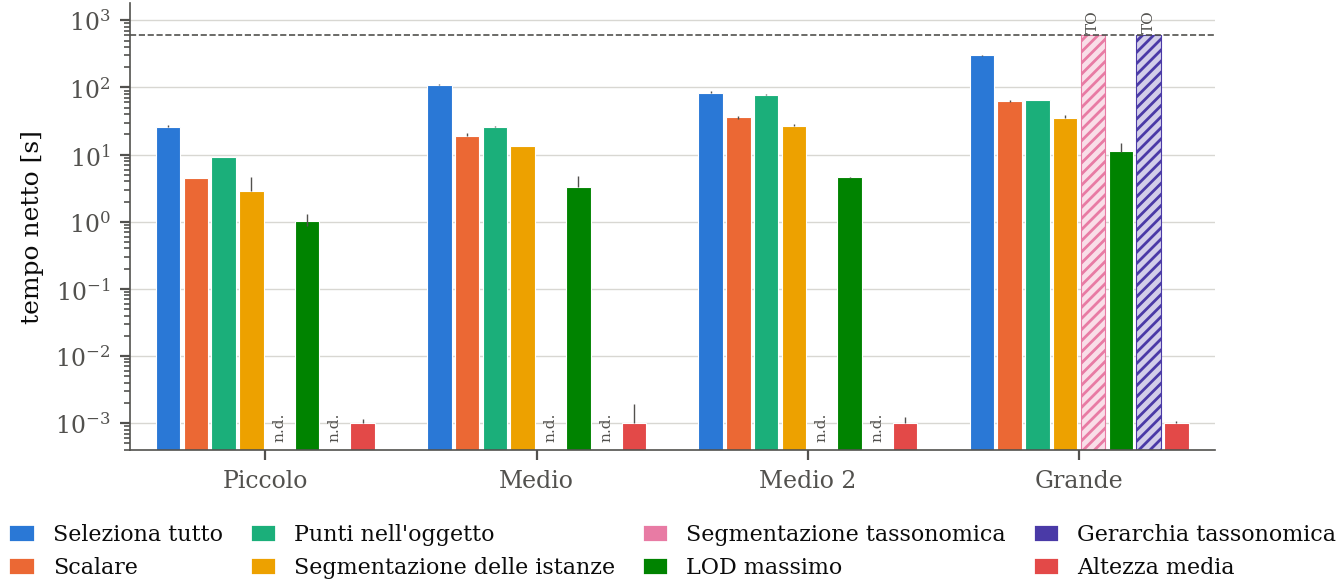
\includegraphics[width=\textwidth]{images/plots/e_oxigraph.png}
    \caption{Oxigraph.}
    \label{fig:e_oxigraph}
  \end{subfigure}
  \caption{Confronto fra le query per singolo motore, raggruppate per dataset (2 di 5). Notazione come nella figura~\ref{fig:engines_1}.}
  \label{fig:engines_2}
\end{figure}

\begin{figure}[htbp]
  \centering
  \begin{subfigure}[b]{\textwidth}
    \centering
    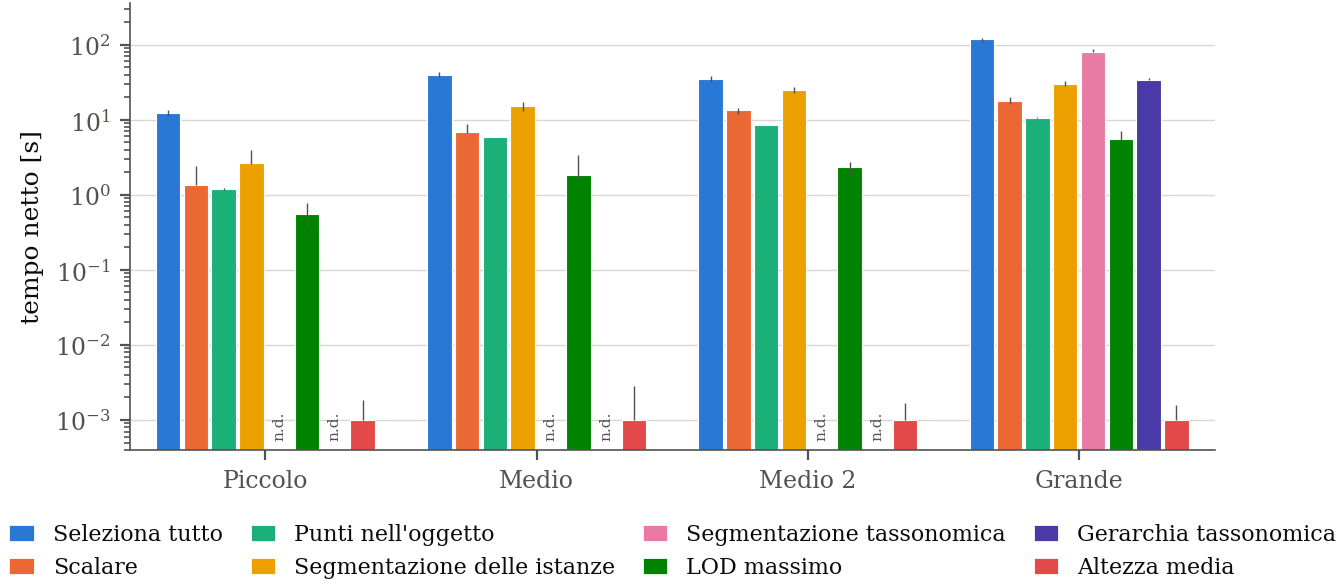
\includegraphics[width=\textwidth]{images/plots/e_qendpoint.png}
    \caption{qEndpoint.}
    \label{fig:e_qendpoint}
  \end{subfigure}
  \\[1.5ex]
  \begin{subfigure}[b]{\textwidth}
    \centering
    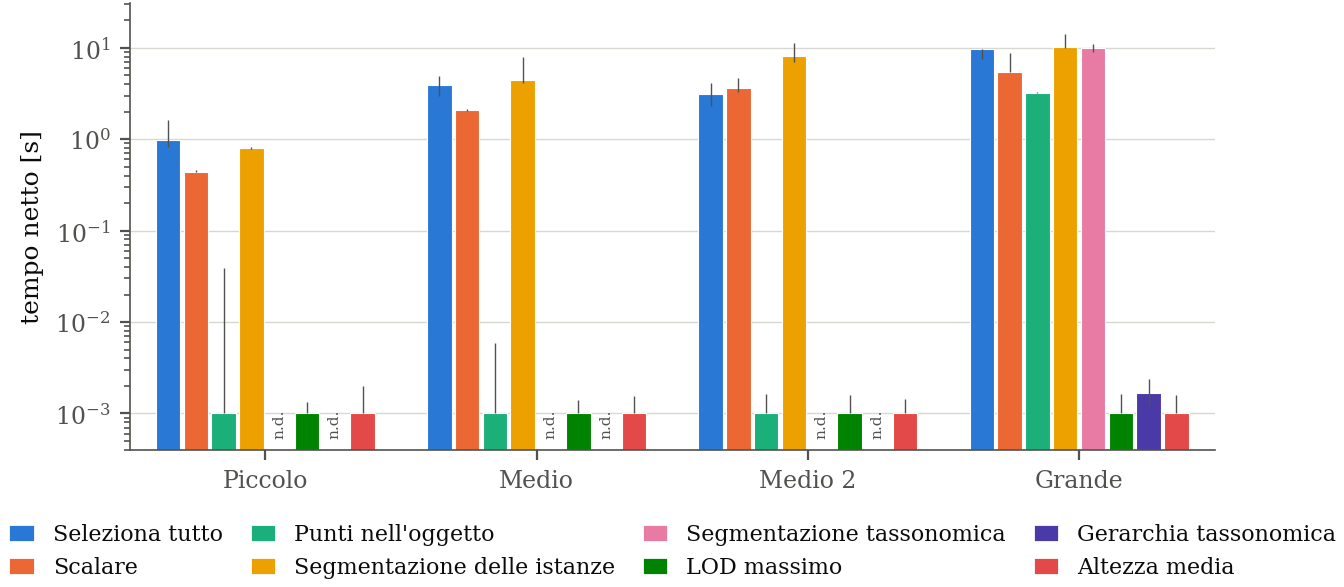
\includegraphics[width=\textwidth]{images/plots/e_qlever.png}
    \caption{QLever.}
    \label{fig:e_qlever}
  \end{subfigure}
  \caption{Confronto fra le query per singolo motore, raggruppate per dataset (3 di 5). Notazione come nella figura~\ref{fig:engines_1}.}
  \label{fig:engines_3}
\end{figure}

\begin{figure}[htbp]
  \centering
  \begin{subfigure}[b]{\textwidth}
    \centering
    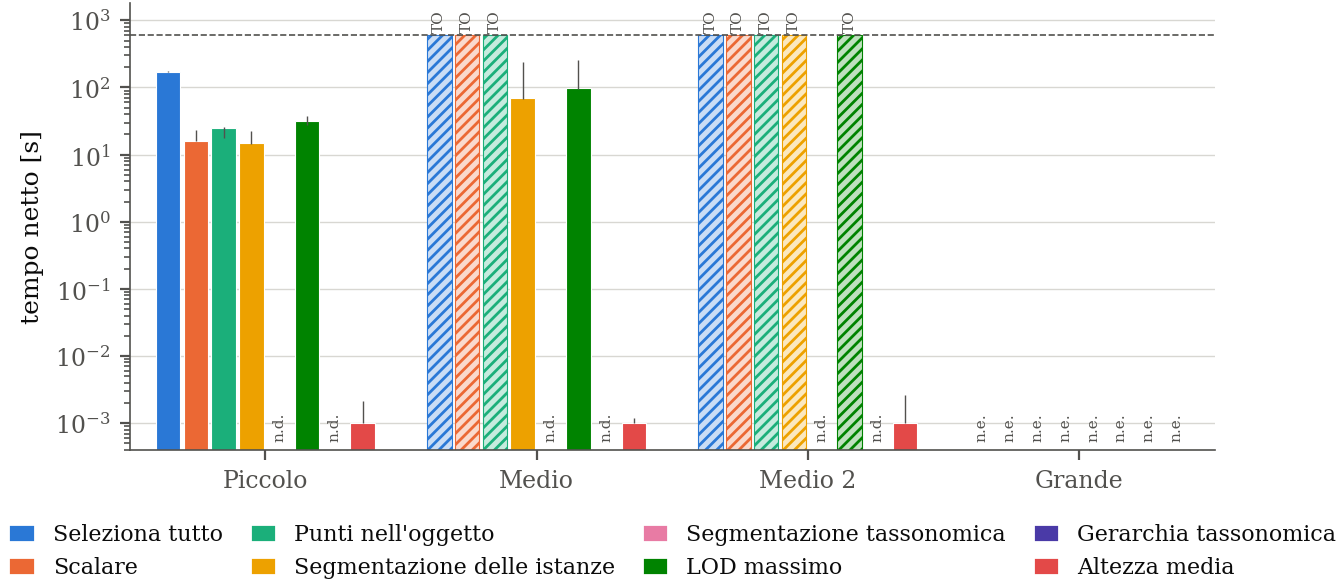
\includegraphics[width=\textwidth]{images/plots/e_rdflib.png}
    \caption{RDFLib.}
    \label{fig:e_rdflib}
  \end{subfigure}
  \\[1.5ex]
  \begin{subfigure}[b]{\textwidth}
    \centering
    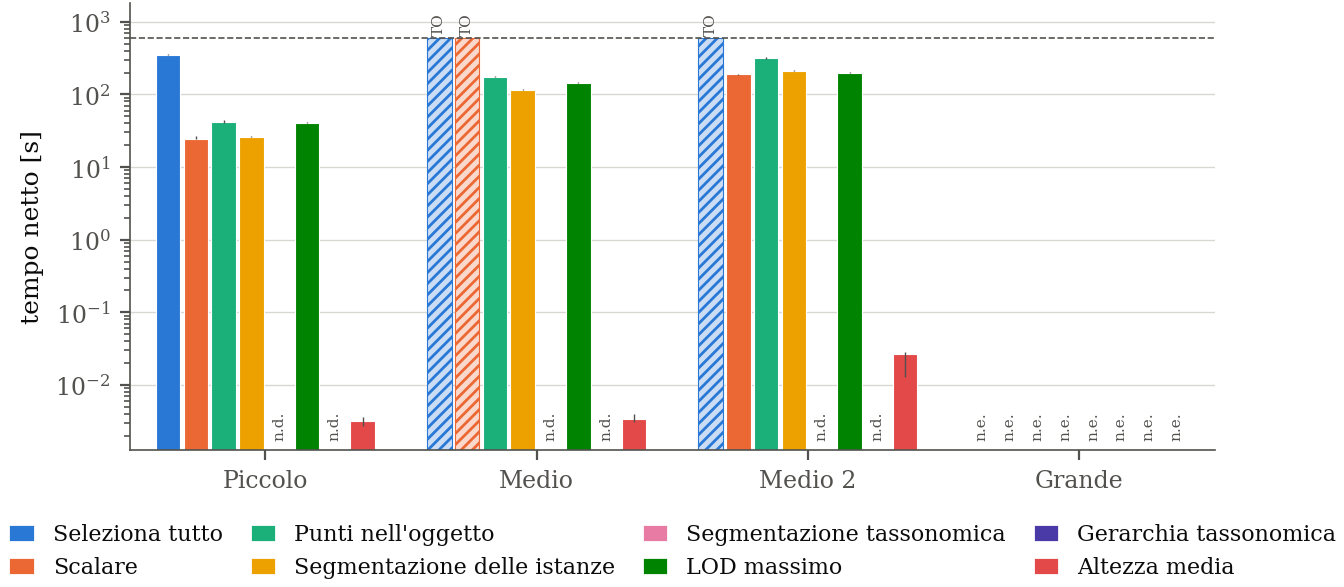
\includegraphics[width=\textwidth]{images/plots/e_rdflib-bdb.png}
    \caption{RDFLib+BDB.}
    \label{fig:e_rdflib-bdb}
  \end{subfigure}
  \caption{Confronto fra le query per singolo motore, raggruppate per dataset (4 di 5). Notazione come nella figura~\ref{fig:engines_1}.}
  \label{fig:engines_4}
\end{figure}

\begin{figure}[htbp]
  \centering
  \begin{subfigure}[b]{\textwidth}
    \centering
    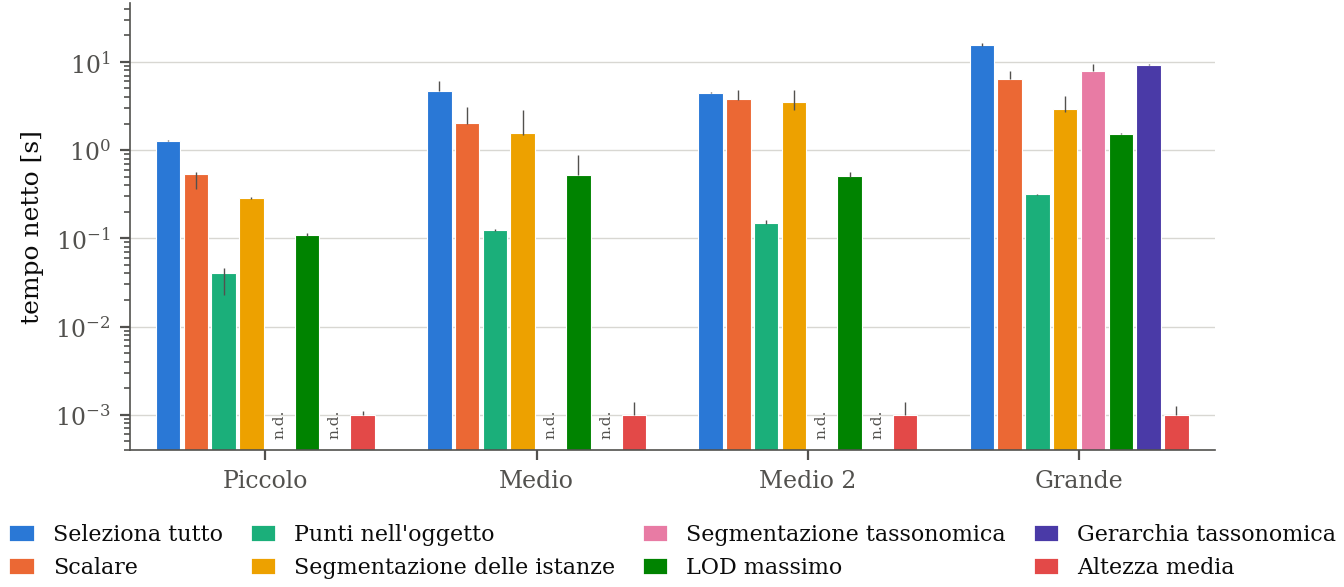
\includegraphics[width=\textwidth]{images/plots/e_rdfox.png}
    \caption{RDFox.}
    \label{fig:e_rdfox}
  \end{subfigure}
  \\[1.5ex]
  \begin{subfigure}[b]{\textwidth}
    \centering
    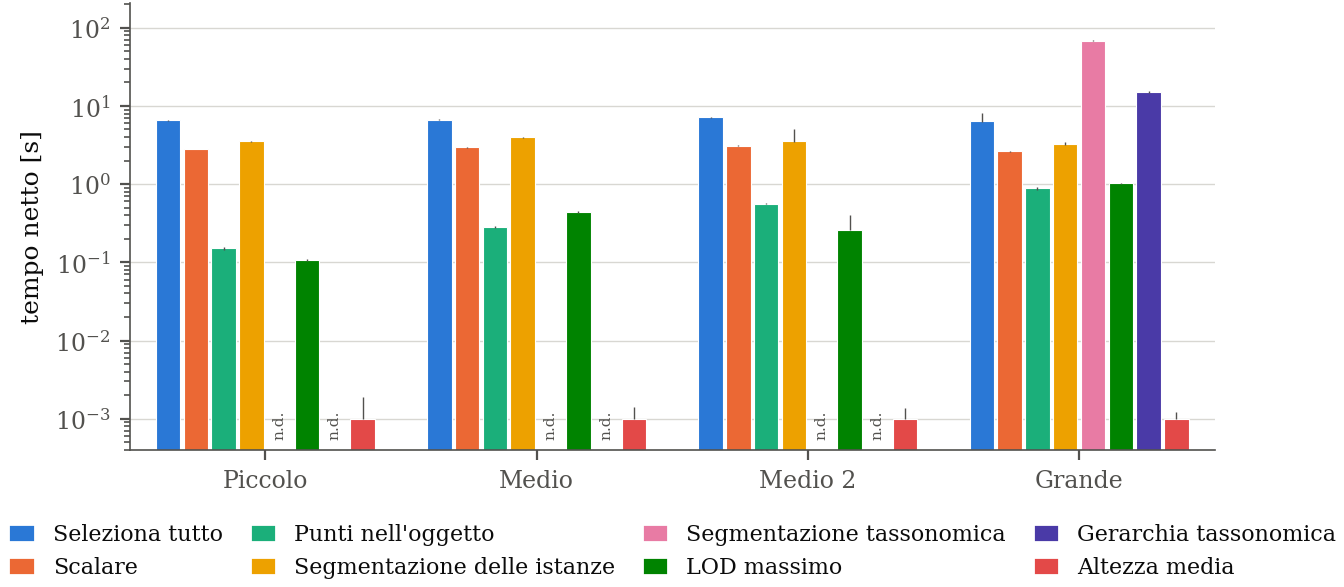
\includegraphics[width=\textwidth]{images/plots/e_virtuoso.png}
    \caption{Virtuoso.}
    \label{fig:e_virtuoso}
  \end{subfigure}
  \caption{Confronto fra le query per singolo motore, raggruppate per dataset (5 di 5). Notazione come nella figura~\ref{fig:engines_1}.}
  \label{fig:engines_5}
\end{figure}

\begin{figure}[htbp]
  \centering
  \begin{subfigure}[b]{\textwidth}
    \centering
    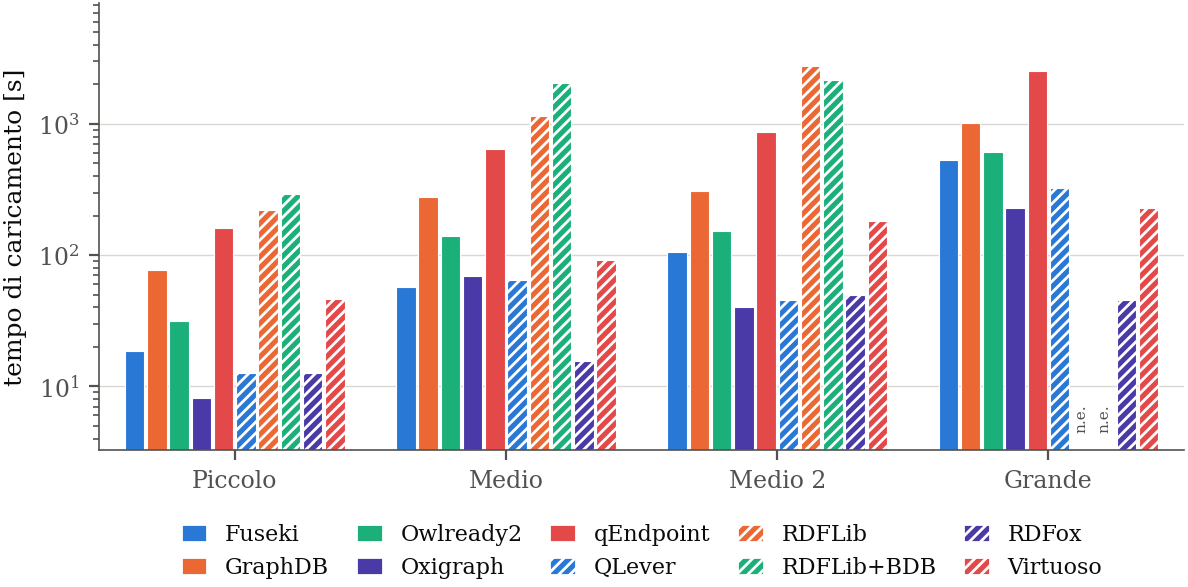
\includegraphics[width=\textwidth]{images/plots/load_time.png}
    \caption{Tempo di caricamento.}
    \label{fig:load_time}
  \end{subfigure}
  \\[1.5ex]
  \begin{subfigure}[b]{\textwidth}
    \centering
    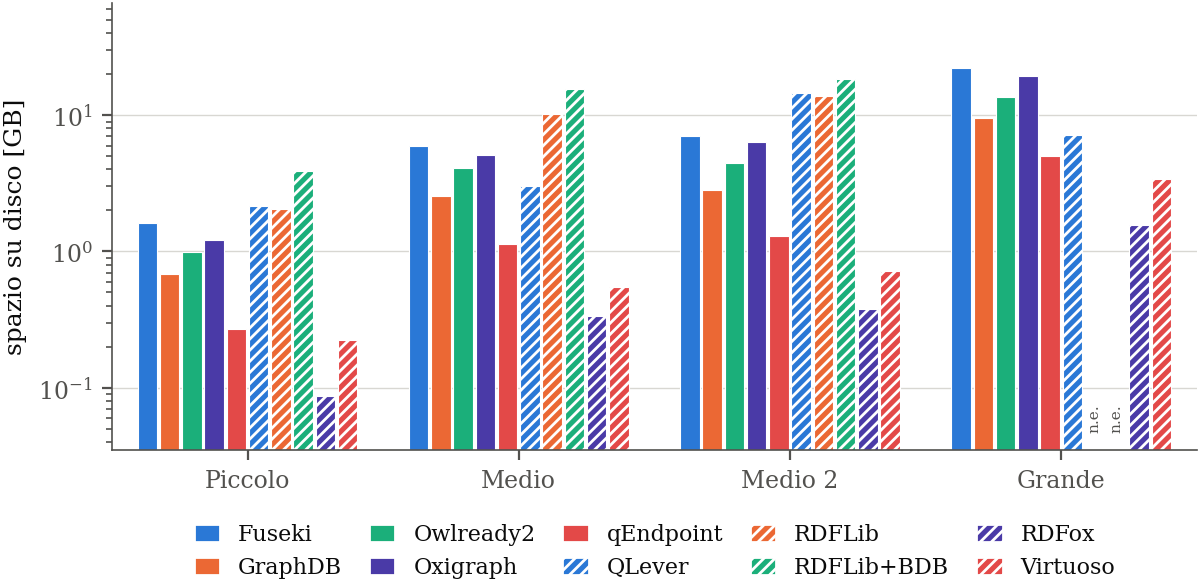
\includegraphics[width=\textwidth]{images/plots/disk_size.png}
    \caption{Spazio occupato su disco.}
    \label{fig:disk_size}
  \end{subfigure}
  \caption{Costo del caricamento dei dataset in ogni motore, in scala logaritmica.}
  \label{fig:loads}
\end{figure}

\begin{figure}[htbp]
  \centering
  \begin{subfigure}[b]{\textwidth}
    \centering
    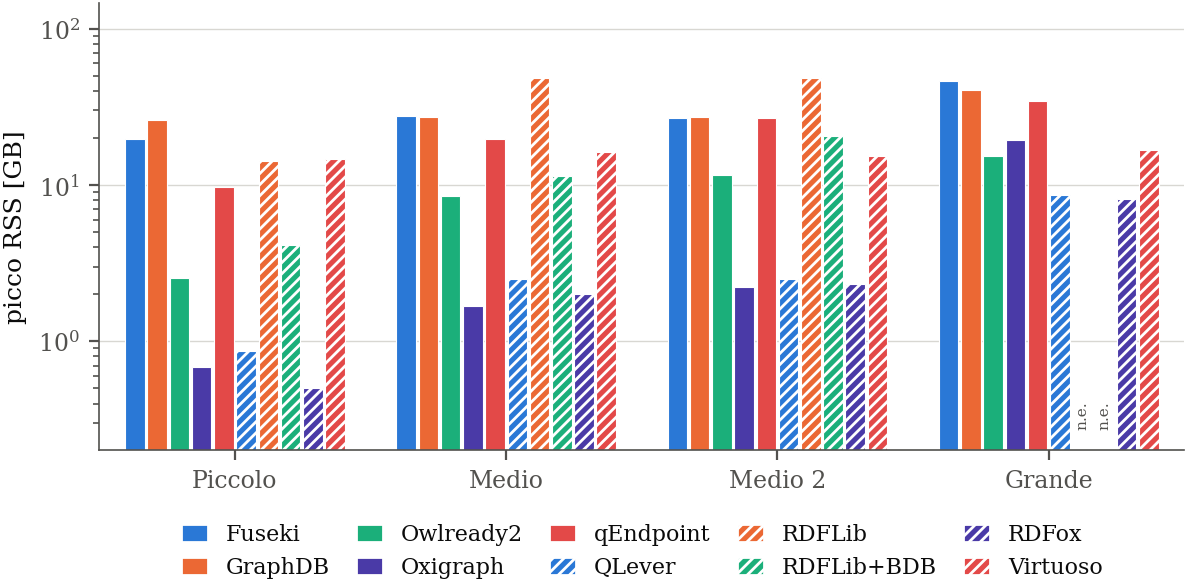
\includegraphics[width=\textwidth]{images/plots/peak_rss.png}
    \caption{Picco di memoria residente, massimo su tutte le query del dataset.}
    \label{fig:peak_rss}
  \end{subfigure}
  \caption{Memoria utilizzata dai motori durante l'esecuzione delle query.}
  \label{fig:memory}
\end{figure}

